\section{Aufbau und Durchführung} % (fold)
\label{sec:aufbau_und_durchf_hrung}

	Zur Messung der ersten beiden Versuchsteile wurden hauptsächlich ein CCD-Detektor und ein Computer mit dem installierten Programm \textit{MaxIm DL Pro 6} verwendet.
	Der CCD-Detektor wurde durch eine vorhandene Kappe abgedunkelt, um es zu ermöglichen Bias- und Dunkelstrombilder aufnehmen zu können und an den Rechner angeschlossen.
	Das Programm ermöglichte die Steuerung der CCD-Kamera und die Verarbeitung von gesendeten Signalen.

	\subsection{Bestimmung des Ausleserauschens des CCD-Detektors} % (fold)
	\label{sub:bestimmung_des_ausleserauschens_des_ccd_detektors}
	
		Das Ausleserauschen des CCD-Detektors wurde mit Hilfe von Bias-Aufnahmen bestimmt.
		Diese entstanden bei geschlossener Blende und sehr kurzer Belichtungszeit und ergeben Bilder, die nur aus dem Biaslevel und zufälligen Rauschen bestehen.
		Um das Biaslevel aufzunehmen, wurden nacheinander einhundert Bias-Aufnahmen bei konstanter Temperatur erstellt, gemittelt und im BIAS-Mean-Bild gespeichert. 
		Die Intensität des zufälligen Rauschens konnte durch Abzug des Bias-Mean von einer willkürlichen Bias-Aufnahme gemessen werden.

	% subsection bestimmung_des_ausleserauschens_des_ccd_detektors (end)


	\subsection{Dunkelstromaufnahme} % (fold)
	\label{sub:dunkelstromaufnahme}

		Hierzu wurde die Blende der CCD geschlossen gehalten und nacheinander bei steigender Temperatur und konstanter Belichtungszeit von 5 Minuten wurden die verschiedenen Dunkelstrombilder erzeugt. 
		Nach Abzug einer anschließend geschossenen BIAS-Aufnahme konnte die Intensität des thermischen Dunkelstromes ermittelt werden.
		Die Einstellung auf die gewünschte Temperatur erfolgte mit Hilfe eines Peltier-Elements.
		Diese erreichen für gewöhnlich Temperaturen von bis zu 30 Grad Celsius unter Umgebungstemperatur.
	% subsection dunkelstromaufnahme (end)


	\subsection{Überprüfung der Linearität} % (fold)
	\label{sub:_berpr_fung_der_linearit_t}
	
		Um den linearen Zusammenhang zwischen eingestrahlter Energie und gemessenen CCD-Signal zu zeigen, wurden Bilder bei stets gleicher Beleuchtung aber von Bild zu Bild steigender Belichtungszeit aufgenommen.
		Die Beleuchtung erfolgte wie in Abbildung \ref{mikrolampe} zu sehen über eine Mikroskoplampe und durch eine Lochblende vor der Kamera um Überbelichtung zu vermeiden.

		\begin{figure}
			\center
			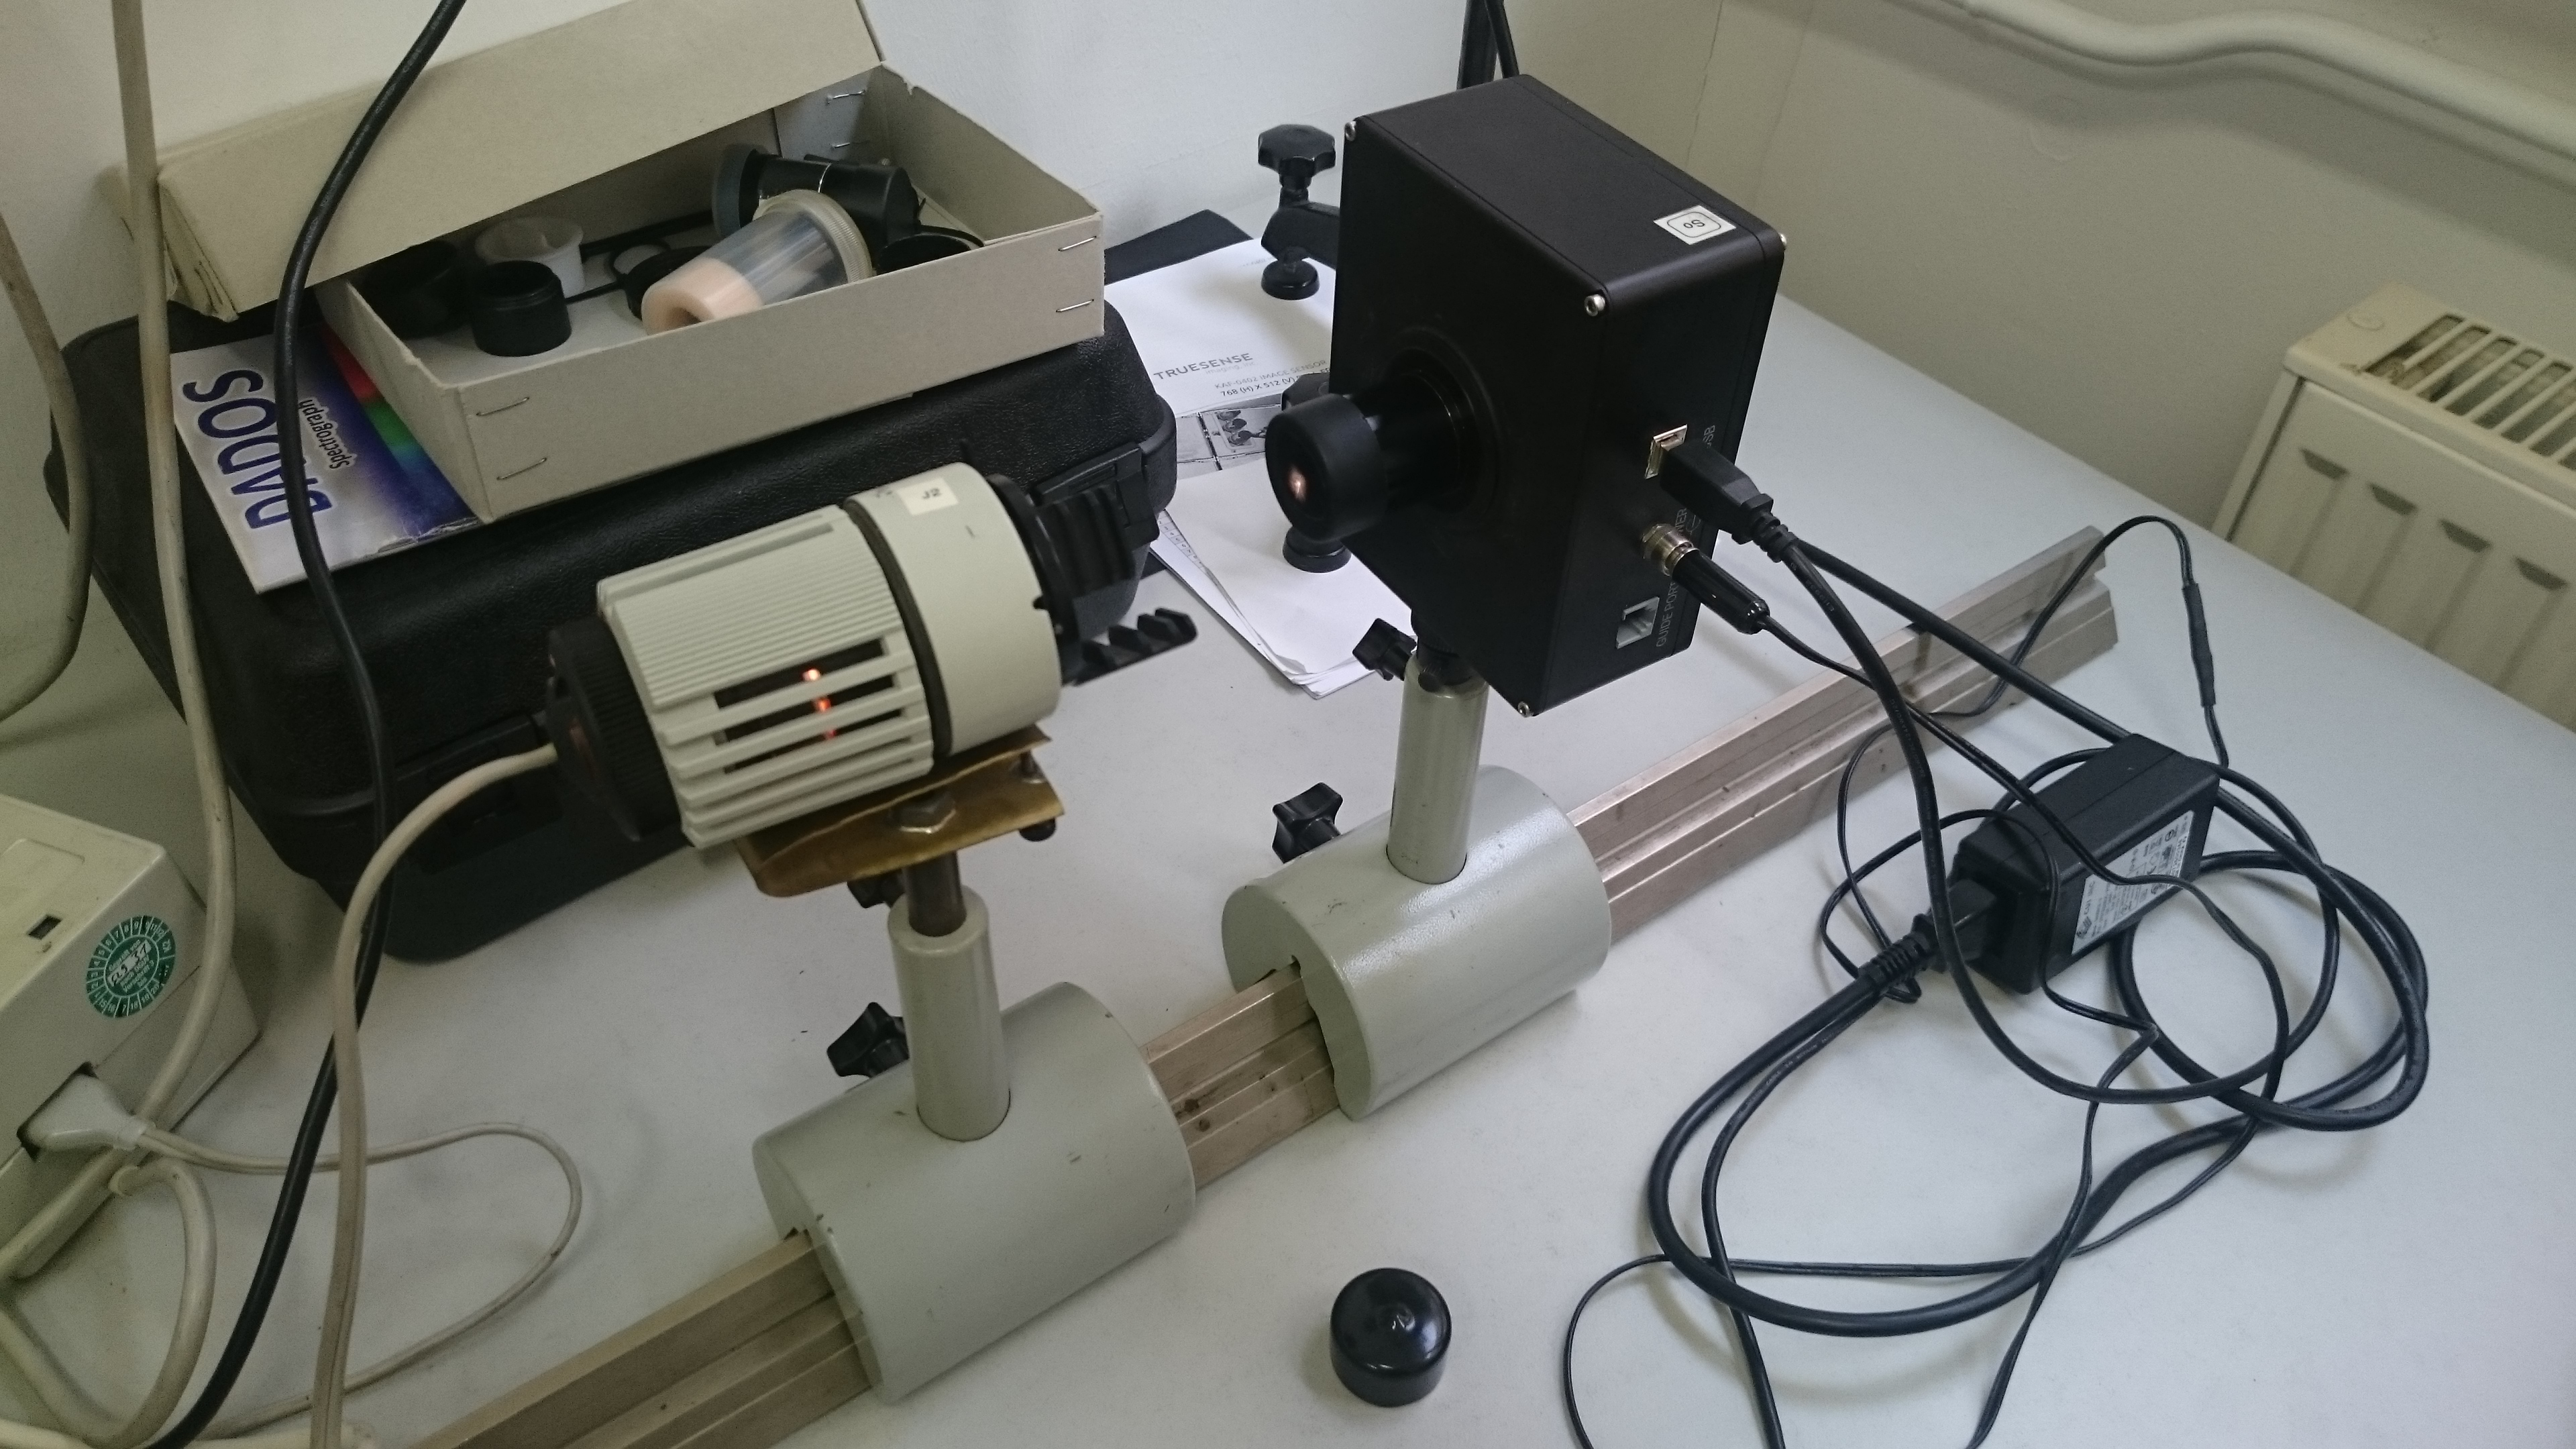
\includegraphics[scale=0.085]{messwerte/Handybilder/DSC_0671.JPG}
			\caption{CCD-Kamera mit beleuchteter Lochblende vor Mikroskoplampe zur Aufnahme der Dunkelstrombilder mit Balsamico und Lachstreifen in Soße Holondaise olé}
			\label{mikrolampe}
		\end{figure}

	% subsection _berpr_fung_der_linearit_t (end)


	\subsection{Kalibrierung des Spektrometers} % (fold)
	\label{sub:kalibrierung_des_spektrometers}
	
	% subsection kalibrierung_des_spektrometers (end)

% section aufbau_und_durchf_hrung (end)